\documentclass[oneside,openany]{tufte-book}

% % %  default French language settings
\usepackage[utf8]{inputenc}	% enable input of accented letters
\usepackage[T1]{fontenc}		% related to above
\usepackage[french]{babel}		% French language support
\usepackage{translator}		% same
	\uselanguage{French}
	\languagepath{French}

\newcommand{\NotDefName}{Ceci n'est pas une définition.}
\newcommand{\NotProofName}{Ceci n'est pas une démonstration.}
\newcommand{\ExampleName}{Ceci est un exemple.}

\usepackage{tcolorbox}

\usepackage{./../styles/style}

%\newcommand{\sidenote}{\footnote}


\title{{\small Ceci n'est pas un manuel d'\newline}algèbre linéaire}
\author{Andr\'e Roberge}
%\publisher{\copyright Andr\'e Roberge \href{https://creativecommons.org/licenses/by-nc-sa/4.0/legalcode.txt}{CC BY-NC-SA-4.0}}

\begin{document}

\maketitle

\hphantom{a}
\vfill
\begin{figure*}
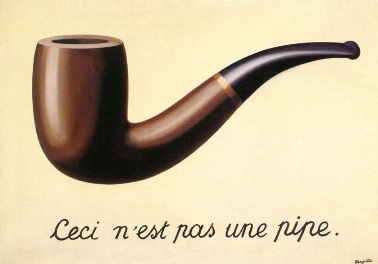
\includegraphics{./../images/MagrittePipe.jpg}
\begin{center}
Par René Magritte
\end{center}
\end{figure*}
\vfill

\tableofcontents
\chapter{Introduction}
Le cours d'introduction à l'algèbre linéaire est souvent
le premier cours au niveau universitaire où les étudiants ont à apprendre des concepts de mathématiques avec une approche
typique de celle utilisée par les mathématiciens professionnels, basée sur l'abstraction et les démonstrations.  Ceci peut être un peu intimidant.

Selon Wikipédia\sidenote{\url{https://fr.wikipedia.org/wiki/Mathématiques}}, les mathématiques sont définies ainsi:

\begin{TrueDef}{Mathématiques}
Les mathématiques (ou la mathématique) sont un ensemble de connaissances abstraites résultant de raisonnements logiques appliqués à des objets divers tels que les nombres, les formes, les structures et les transformations. Elles sont aussi le domaine de recherche développant ces connaissances, ainsi que la discipline qui les enseigne.

Elles possèdent plusieurs branches telles que : l'arithmétique, l'algèbre, l'analyse, la géométrie, la logique mathématique, etc. Il existe également une certaine séparation entre les mathématiques pures et les mathématiques appliquées.
\end{TrueDef}

Dans ce livre, nous présentons les définitions formelles
dans des encadrés en bleu tel que celui ci-dessus. 
Un des buts de ce manuel est de vous aider à développer
une compréhension intuitive de certaines définitions
que l'on retrouve en algèbre linéaire.
Pour vous aider, nous allons souvent utiliser en premier
des définitions un peu plus informelles.  Par exemple, votre expérience dans vos cours de mathématiques vous fait
peut-être penser que la définition des mathématiques ressemble plutôt à la suivante:

\begin{NotDef}
Les mathématiques qu'on voit au niveau universitaire
ont été inventés par des sadiques qui inventent des
termes compliqués\sidenote{Comme le "non-sens abstrait" \url{https://fr.wikipedia.org/wiki/Abstract_nonsense}} uniquement dans le but de décourager les étudiants.
\end{NotDef}



\section{Au sujet des démonstrations}

Les mathématiciens \textbf{adorent} les démonstrations\sidenote{Certains utilisent parfois le mot \textit{preuve} au lieu de démonstration, ce qui est un anglicisme.}.
Le but de ce manuel est de vous donner une idée intuitive
des concepts de base de l'algèbre linéaire en évitant les démonstrations. Cependant, nous utilisons
généralement des exemples simples pour guider votre intuition\sidenote{Nous incluons parfois des énoncés qui peuvent être faux dans un contexte différent.}.

\begin{NotProof}
Un exemple n'est pas une démonstration. Un argument de plausibilité n'est pas une démonstration. Une démonstration
est une suite précise de propositions logiques. Le manuel recommandé par votre professeur contient toutes les démonstrations requises.
Votre professeur inclut des démonstrations à faire dans les
examens uniquement\sidenote{Ceci n'est pas toujours vrai; 
ça dépend du professeur qui enseigne le cours} dans le but de faire baisser votre note dans le cours.
\end{NotProof}

Les notes en marge\sidenote{Comme celle-ci.} ajoutent des
détails que vous trouverez parfois utile\sidenote{Du moins, je l'espère.}.

\section{Au sujet des exemples}

En général, je cherche à choisir des exemples tellement simples qu'ils sont probablement jugés par votre professeur comme l'étant beaucoup trop pour être utilisé en classe,
ou dans votre manuel de cours. Il est vrai que, très souvent,
les exemples que j'ai choisis peuvent cacher la complexité
d'un sujet donné: vous devriez les considérer comme un
simple premier pas dans votre voyage d'apprentissage du sujet.

\chapter{Systèmes d'équations linéaires}
Considérez l'équation suivante:
\[
x = 2
\]
Ceci est une équation linéaire avec une seule inconnue.

\begin{NotDef}
Une \textbf{inconnue} est un \textit{scalaire} déguisé sous
la forme d'une lettre\sidenote{Pour augmenter la confusion, on utilise parfois des lettres
grecques au lieu de lettre de l'alphabet latin utilisé en
français.}.

Un \textbf{scalaire} est le mot utilisé en mathématiques
supérieures pour désigner un nombre\sidenote{Dans ce livre, on suppose toujours que c'est un nombre réel.}.
\end{NotDef}

Rajoutons une deuxième équation linéaire, avec une autre
inconnue.
\[
\left\{
\begin{matrix}
    x &=& 2\\
    y &=& 1
\end{matrix}
\right.
\]
\begin{marginfigure}
\begin{mdframed}
    \scalebox{0.8}{
		\begin{tikzpicture}
			% les axes
			\draw[->] (-1,0) -- (4,0) node[anchor=west]{\color{gray}x};
			\draw[->] (0,-1) -- (0,4) node[anchor=south]{\color{gray}y};
			% les deux droites
			\draw[-, thick, blue] (-1,1) -- (4,1) node[anchor=north]{\color{blue}\small $y=1$};
			\draw[-, thick, purple] (2,-1) --(2,4) node[anchor= east]{\color{purple}\small $x=2$};
			% le point d'intersection
			\coordinate (A) at (2,1);
			\draw[-] (2, -0.1) node[anchor=north]{\small 2} -- (2, 0.1);
			\draw[-] (-0.1, 1) node[anchor=east]{\small 1} -- (0.1, 1);
			\node [fill=black,inner sep=2pt,label=30:$\mbox{\quad(2,1)}$] at (2,1) {};
		\end{tikzpicture}
}
\caption{Deux droites qui s'intersectent dans un plan.}
\end{mdframed}
\end{marginfigure}

Ceci est un exemple d'un \textbf{système} d'équations linéaires.

\begin{NotDef}
Un \textbf{système d'équations linéaires} est une collection
d'équations linéaires ayant des inconnues communes.%
\sidenote{Pour que l'utilisation du mot \textit{communes} soit correct, il faudrait
plutôt écrire:
\[
\left\{
\begin{matrix}
    x + 0y &=& 2\\
    y + 0x &=& 1
\end{matrix}
\right.
\]
}
\end{NotDef}

Puisqu'on a un système avec deux inconnues, $x$ et $y$, on
peut le représenter par deux droites dans un plan.
La \textbf{solution} de ce système correspond au point
d'intersection de ces deux droites.

Algébriquement, on peut représenter cette solution de deux
façons:
\begin{itemize}
\item[$\bullet$] En utilisant la notation traditionnelle
pour un point: $(x, y) = (2, 1)$.
\item[$\bullet$] En écrivant la solution comme un système
d'équations linéaires où chaque inconnue n'apparait qu'une
seule fois, avec une ligne différente pour chaque inconnue. 
Ceci est identique à ce que nous avions écrit précédemment:
\[
\left\{
\begin{matrix}
    x &=& 2\\
    y &=& 1
\end{matrix}
\right.
\]
\end{itemize}

\section{Opérations élémentaires sur les lignes}

Le système d'équations linéaires que nous avons écrit
ci-dessus comporte deux équations, chacune écrite sur
une ligne différente. Nous pouvons numéroter ces équations
dans l'ordre où elles apparaissent.
\[
\left\{
\begin{matrix}
    x &=& 2\qquad {\scriptstyle\color{red}\fbox{1}}\\
    y &=& 1 \qquad {\scriptstyle\color{red}\fbox{2}}
\end{matrix}
\right.
\]
Nous pouvons interchanger les deux lignes sans que 
la solution ne change
\[
\left\{
\begin{matrix}
    y &=& 1\qquad {\scriptstyle\color{red}\fbox{1}}\\
    x &=& 2 \qquad {\scriptstyle\color{red}\fbox{2}}
\end{matrix}
\right.
\]
On dit que ces deux systèmes d'équations linéaires\sidenote{L'original et celui avec les équations dans un autre ordre différent.}
sont \textbf{équivalents}.
\begin{TrueDef}{Équivalence}
Deux systèmes d'équations linéaires sont dits \textbf{équivalents} s'ils ont la même solution.
\end{TrueDef}
L'interchange de deux lignes est un exemple
d'une \textbf{opération élémentaire sur les lignes}.
Dans ce qui suit, on dénotera un tel interchange
de la façon suivante:
\[
L_1 \leftrightarrow L_2
\]

\begin{NotDef}
Une \textbf{opération élémentaire sur les lignes}\footnote{Une opération élémentaire sur les lignes n'est pas un concept mathématique mais un truc de calcul; il n'y a
donc pas de définition formelle pour ceci.} est
une opération mathématique qui transforme un système
d'équations linéaires en un système équivalent.
\end{NotDef}

Une autre opération sur les lignes qu'on peut effectuer est
de remplacer une ligne donnée par l'addition de celle-ci avec le multiple 	d'une autre ligne.


\begin{align*}
&\left\{
\begin{matrix}[ccc]
    y&=& 1\qquad {\scriptstyle\color{red}\fbox{1}}\\
    x &=& 2\qquad {\scriptstyle\color{red}\fbox{2}}
\end{matrix}
\right.
\\
&\qquad\mbox{\color{blue} est équivalent à}\\
&\left\{
\begin{matrix}[rrrrll]
    &&y&=& 1	\\	
    x&-&y &=& 1 & {\color{blue}\Leftarrow\quad L_2 - L_1} 
\end{matrix}
\right.
\end{align*}
		

Finalement, une troisième opération élémentaire qu'on peut effectuer
est de multiplier une ligne par une constante différente
de zéro.

\begin{align*}
&\left\{
\begin{matrix}[rrrrl]
    &&y&=& 1	\qquad {\scriptstyle\color{red}\fbox{1}}\\	
    x&-&y &=& 1\qquad {\scriptstyle\color{red}\fbox{2}}
\end{matrix}
\right.
\\
&\qquad\mbox{\color{blue} est équivalent à}\\
&\left\{
\begin{matrix}[rrrrll]
    &&3y&=& 3	&{\color{blue}\Leftarrow\quad 3 L_1}\\	
    x&-&y &=& 1
\end{matrix}
\right.
\end{align*}

Pour vraiment compliquer les choses davantages,
faisons une dernière opération sur les lignes
\begin{marginfigure}
		\begin{tikzpicture}
			% les axes
			\draw[->] (-1,0) -- (4.2,0) node[anchor=west]{\color{gray}x};
			\draw[->] (0,-1) -- (0,4) node[anchor=south]{\color{gray}y};
			% les deux droites
			\draw[-, thick, blue] (0,-1) -- (4,3) node[anchor=east]{\color{blue}\small $x-y=1$};
			\draw[-, thick, purple] (-1,2.5) --(4.2,-0.1) node[anchor=north]{\color{purple}\small $x+2y=4$};
			% le point d'intersection
			\coordinate (A) at (2,1);
			\draw[-] (2, -0.1) node[anchor=north]{\small 2} -- (2, 0.1);
			\draw[-] (-0.1, 1) node[anchor=east]{\small 1} -- (0.1, 1);
			\draw [dashed, gray] (2, 0.2) -- (A);
			\draw [dashed, gray] (0.2, 1) -- (A);
			\node [fill=black,inner sep=2pt,label=0:$\mbox{\quad(2,1)}$] at (2, 1) {};
		\end{tikzpicture}
			\caption{Interprétation graphique de ce nouveau système d'équations linéaires}
\end{marginfigure}

\begin{align*}
&\left\{
\begin{matrix}[rrrrl]
    &&3y&=& 3	\qquad {\scriptstyle\color{red}\fbox{1}}\\	
    x&-&y &=& 1\qquad {\scriptstyle\color{red}\fbox{2}}
\end{matrix}
\right.
\\
&\qquad\mbox{\color{blue} est équivalent à}\\
&\left\{
\begin{matrix}[rrrrll]
    x&+&2y&=& 4	&{\color{blue}\Leftarrow\quad L_1 + L_2}\\	
    x&-&y &=& 1
\end{matrix}
\right.
\end{align*}
Bien que les deux équations soient très différentes de celles
du départ, et que le graphique correspondant soit également
différent, la solution reste inchangée.

Nous avons donc maintenant un système d'équations linéaires avec deux inconnues, où les deux inconnues apparaissent dans chacune des deux équations. Ce système est équivalent à celui du départ, plus simple et où on peut immédiatement identifier
la valeur de chacune des inconnues.

\[
\left.
\begin{matrix}
    x &=& 2\\
    y &=& 1
\end{matrix}
\right\} \qquad\mbox{équivalent à}\qquad 
\left\{
\begin{matrix}
    x&+&2y&=& 4	\\	
    x&-&y &=& 1
\end{matrix}
\right.
\]
\section{Matrice augmentée}

\begin{NotDef}
Une \textbf{inconnue} est un scalaire qui s'est déguisée sous
la forme d'une lettre, \textit{parfois augmentée d'un \textbf{indice}, et
dont on demande aux étudiants d'en deviner l'identité.}

Un \textbf{indice} est un chiffre qu'on met au bas d'une lettre, comme
ceci: $x_{\color{red} 1}$,
pour la distinguer d'une autre lettre, $x_{\color{red} 2}$, identique mais indiquant une quantité différente; on utilise
parfois un indice lorsqu'on pense qu'on n'a pas
suffisamment de lettres dans l'alphabet pour
désigner toutes les inconnues.\sidenote{Il ne faut pas
confondre un indice, et un \textbf{exposant}, ce dernier apparaissant
en haut de la lettre, $x^1$.}
\end{NotDef}

Supposons que l'on vous demande de trouver la
solution du système d'équations linéaires suivant:
\[
\left\{
\begin{matrix}
    x_1&+&2x_2&=& 4	\\	
    x_1&-&x_2 &=& 1
\end{matrix}
\right.
\]
ayant les inconnues $x_1$ et $x_2$.  Sauf pour le choix
des inconnues, on reconnait ce système d'équations linéaires
comme étant identique au précédent. On connait donc déjà la
solution:
\[
\left\{
\begin{matrix}
x_1 &=& 2\\
x_2 &=& 1
\end{matrix}
\right.
\]
Si on ne connaissait pas cette solution, on aurait pu la
retrouver en faisant l'inverse des opérations élémentaires
sur les lignes qu'on avait vu\sidenote{On fera ceci dans
un exemple ci-dessous.}.
Parce que ces opérations élémentaires ne dépendent pas des
choix des symboles utilisés pour dénoter les inconnues,
on trouve utile d'introduire une notation qui n'inclut pas
ces symboles. Ainsi, au lieu d'écrire:
\[
\left\{
\begin{matrix}
    x_1&+& 2x_2&=& 4	\\	
    x_1&-&x_2 &=& 1
\end{matrix}
\right.
\color{black}
\]
on écrit la version totalement équivalente suivante:
\[
\left\{
\begin{matrix}
    {\color{red}1}x_1&+& {\color{red}2}x_2&=& {\color{blue}4}	\\	
    {\color{red}1}x_1&+&({\color{red}-1})x_2 &=& {\color{blue}1}
\end{matrix}
\right.
\color{black}
\]
Les chiffres, en rouge, devant les inconnues sont appelés
les \textbf{coefficients}; ceux en bleu sont les termes constants.
Ayant identifié les coefficients et les termes constants,
on se débarrasse de tout le reste, considéré comme une notation
superflue, et on écrit plutôt:
\[
\begin{bmatrix}[rr|r]
{\color{red}1} & {\color{red}2} & {\color{blue}4}\\
{\color{red}1} & {\color{red}-1} & {\color{blue}1}
\end{bmatrix}
\]
On appelle ceci la \textbf{matrice\sidenote{On verra la définition d'une matrice dans le prochain chapitre} augmentée} du système
d'équations linéaires. La partie à gauche de la barre verticale\sidenote{Certains mathématiciens, préférant le minimalisme absolu, n'incluent pas
une telle barre verticale dans une matrice augmentée.}, 
avec les chiffres en rouge, s'appelle \textbf{matrice des coefficients}. 

\begin{NotDef}
La notation des matrices augmentées a été inventée par des mathématiciens qui cherchaient à trouver des solutions
pour des systèmes d'équations linéaires mais qui n'aimaient
pas utiliser des lettres (pour les inconnues), ni des signes
d'addition ($+$) ou d'égalité ($=$).
\end{NotDef}

On peut également écrire la solution sous la forme
d'une matrice augmentée en procédant comme ceci:
\[
\left\{
\begin{matrix}
x_1 &=& 2\\
x_2 &=& 1
\end{matrix}
\right.
\quad {\color{purple}\Rightarrow}\quad
\left\{
\begin{matrix}
{\color{red}1} x_1 &+& {\color{red}0}x_2 &=& {\color{blue}2}\\
{\color{red}0} x_1 &+& {\color{red}1}x_2 &=& {\color{blue}1}
\end{matrix}
\right.
\quad {\color{purple}\Rightarrow}\quad
\begin{bmatrix}[rr|r]
{\color{red}1} & {\color{red}0} & {\color{blue}2}\\
{\color{red}0} & {\color{red}1} & {\color{blue}1}
\end{bmatrix}
\]

La matrice augmentée de la solution est dans ce qu'on
appelle une \textit{forme échelonnée réduite} que l'on définira un peu plus tard.

Dans un cours d'introduction à l'algèbre linéaire, \textbf{la très grande majorité des calculs\sidenote{Ce qui semble ëtre difficile pour les étudiants est d'interpréter correctement ces calculs qui sont,
en général, très simples.} que vous aurez
à faire} consiste à faire des opérations élémentaires sur les lignes
pour obtenir, si cela est possible, une matrice
\textbf{équivalente} dans la \textbf{forme échelonnée réduite.}

\begin{Example}
\[
\begin{matrix}
\color{blue}\left\{
\begin{matrix}[rrrrr]
x_1 &+& 2x_2 &=& 4\\
x_1 & -& x_2 &=& 1
\end{matrix} \right. &\color{blue}\Rightarrow&
\begin{bmatrix}[rr|r]
1 & 2 & \hphantom{-}4\\
1 & -1 & 1
\end{bmatrix} \\[20pt]
\color{red}L_2 - L_1 \rightarrow L_2 &\color{red}\Rightarrow&
\begin{bmatrix}[rr|r]
1 & 2 & 4\\
0 & -3 & -3
\end{bmatrix} \\[20pt]
\color{red}-\frac13 L_2 \rightarrow L_2 &\color{red}\Rightarrow&
\begin{bmatrix}[rr|r]
1 & \hphantom{-}2 & \hphantom{-}4\\
0 & 1 & 1
\end{bmatrix} \\[20pt]
\color{red}L_1 - 2L_2 \rightarrow L_1 &\color{red}\Rightarrow&
\begin{bmatrix}[rr|r]
1 & \hphantom{-}0 & \hphantom{-}2\\
0 & 1 & 1
\end{bmatrix} &\color{blue}\Rightarrow&
\color{blue}\left\{
\begin{matrix}
x_1 &=& 2\\
x_2 &=& 1
\end{matrix}
\right.
\end{matrix}
\]
\end{Example}

Nous terminons ce chapitre avec deux véritables définitions mathématiques.

\begin{TrueDef}{Équation linéaire}
Une \textbf{équation linéaire} est une équation qu'on peut mettre sous la forme
\[
a_1 x_1 + \ldots + a_n x_n = b
\]
où $b$ ainsi que les coefficients $a_1, \ldots a_n$ sont
des scalaires connus, et $x_1, \ldots, x_n$ sont des
inconnues.
\end{TrueDef}

\begin{TrueDef}{Système d'équations linéaires}
Un système de d'équations linéaires est une
collection de $m$ équations linéaires qui portent
sur les mêmes $n$ inconnues:
\[
\left\{
	\begin{matrix}
	a_{11}x_1 &+& a_{12}x_2 &+& \ldots &+& a_{1n}x_n &=& b_1 \\
	a_{21}x_1 &+& a_{22}x_2 &+& \ldots &+& a_{2n}x_n &=& b_2 \\
	\vdots && \vdots &&  && \vdots && \vdots \\
	a_{m1}x_1 &+& a_{m2}x_2 &+& \ldots &+& a_{mn}x_n &=& b_m
	\end{matrix}
	\right.
\]
\end{TrueDef}


\chapter{Matrices}
Sans avoir défini ce qu'était une \textbf{matrice}, nous avons
néanmoins introduit un objet appelé \textbf{matrice augmentée}.
Sans plus attendre, voici une définition formelle d'une \textbf{matrice}.

\begin{TrueDef}{Matrice}
Soit $m$ et $n$ deux entier positifs; une matrice de \textbf{taille}
$m\times n$
est une collection de $mn$ nombres, appelés coefficients, arrangés dans un tableau rectangulaire:
\[
\begin{matrix}[cc]
&\text{$n$ colonnes} \\
\text{$m$ lignes}& \begin{pmatrix}
        a_{11} & a_{12} & \ldots & a_{1n}\\
        a_{21} & a_{22} & \ldots & a_{2n}\\
        \vdots & \vdots & \vdots & \vdots \\
        a_{m1} & a_{m2} & \ldots & a_{mn}
        \end{pmatrix}
  \end{matrix}
\]
\end{TrueDef}

Vous avez peut-être remarqué\sidenote{
Croyez-le ou non, ceci n'est pas une coïncidence.} que la notation utilisée pour
les coefficients dans la définition
d'une matrice ressemble étrangement à celle utilisée dans la définition d'un système d'équations linéaires.

\begin{TrueDef}{Système d'équations linéaires}
Un système de d'équations linéaires est une
collection de $m$ équations linéaires qui portent
sur les mêmes $n$ inconnues:
\[
\left\{
	\begin{matrix}
	a_{11}x_1 &+& a_{12}x_2 &+& \ldots &+& a_{1n}x_n &=& b_1 \\
	a_{21}x_1 &+& a_{22}x_2 &+& \ldots &+& a_{2n}x_n &=& b_2 \\
	\vdots && \vdots &&  && \vdots && \vdots \\
	a_{m1}x_1 &+& a_{m2}x_2 &+& \ldots &+& a_{mn}x_n &=& b_m
	\end{matrix}
	\right.
\]
\end{TrueDef}

\begin{Example}
Voici une matrice de taille $2 \times 3$:
\[\begin{bmatrix} 2 & 1 & 0 \\ 1 & 3 & 5 \\ \end{bmatrix}\]

Au lieu d'utiliser des crochets, $[\ldots]$,
  on utilise parfois des parenthèses pour encadrer les coefficients d'une matrice:
  \[\begin{pmatrix} 2 & 1 & 0 \\ 1 & 3 & 5 \\ \end{pmatrix}\]
\end{Example}

Nous allons étudier plusieurs propriétés des matrices dans ce
livre. Pour l'instant, nous allons nous limiter à définir deux
\textit{formes} que peuvent prendre les matrices. 


\section{Matrice de forme échelonnée}

%%%%%%%%%%%%%%%%%%%%%%%%

La matrice suivante est dans la \textbf{forme échelonnée}:
\[
\begin{bmatrix}[ccccccccc]
p_1 & *  & * & * & * & * & * & * & * \\
0 & 0 & p_2 & * & * & * & * & * & * \\
0 & 0 & 0 & p_3 & * & * & * & * & * \\ 
0 & 0 & 0 & 0 & 0 & 0 & p_4 & * & * \\ 
0 & 0 & 0 & 0 & 0 & 0 & 0 & 0 & p_5 
\end{bmatrix}
\]
Dans cette matrice, les coefficients $p_1, p_2, \ldots$
sont tous différents de zéro. De plus, les coefficients
identifiés par un astérisque, $*$, peuvent prendre n'importe
quelle valeur. 
Une matrice est en forme échelonnée si
le premier coefficient non-nul d'une ligne donnée est toujours à 	la droite du coefficient non-nul de la ligne précédente. On appelle
ce coefficient non-nul un \textbf{pivot}. Pour aider à identifier
ce qu'on entent par une forme échelonnée, nous écrivons la matrice
à nouveau mais, cette fois, nous 
identifions une forme en escalier\sidenote{C'est à cette
forme en escalier que le mot \textit{échelonné} fait
référence.} sous laquelle tous
les coefficients doivent être nuls.
\[
\newcommand*{\temp}{\multicolumn{1}{c|}{\color{red}0}}
\begin{bmatrix}[ccccccccc]
p_1 & * & *  & * & * & * & * & * & * \\ \cline{1-2}
\color{red}0 & \temp & p_2 & * & * & * & * & * & *  \\ \cline{3-3}
\color{red}0 &\color{red}0 & \temp & p_3 & * & * & * & * & * \\ \cline{4-6}
\color{red}0 &\color{red}0 & \color{red}0 & \color{red}0 & \color{red}0 & \temp & p_4 & * & * \\ \cline{7-8}
\color{red}0 &\color{red}0 & \color{red}0 &\color{red}0 & \color{red}0 & \color{red}0 & \color{red}0 & \temp & p_5 
\end{bmatrix}
\]
Une matrice est dans la forme échelonnée \textbf{réduite} si,
en plus d'être dans une forme échelonnée, tous les pivots
sont égaux à 1, et tous les autres coefficients dans un colonne
où il y a un pivot, sont égaux à 0.

\[
\newcommand*{\tempr}{\multicolumn{1}{c|}{\color{red}0}}
\newcommand*{\tempb}{\multicolumn{1}{c|}{\color{blue}0}}
\begin{bmatrix}[ccccccccc]
\mbox{\large{\textcircled{\small $1$}}} & * & \color{blue}0 & \color{blue}0 & * & * & \color{blue}0 & * & \color{blue}0 \\ \cline{1-2}
\color{blue}0 &\tempr & \mbox{\large{\textcircled{\small $1$}}} & \color{blue}0 & * & * & \color{blue}0 & * & \color{blue}0 \\ \cline{3-3}
\color{blue}0 &\color{red}0 &  \tempb & \mbox{\large{\textcircled{\small $1$}}} & * & * & \color{blue}0 & * & \color{blue}0 \\ \cline{4-6}
\color{blue}0 &\color{red}0 & \color{blue}0 & \color{blue}0 & \color{red}0 & \tempr & \mbox{\large{\textcircled{\small $1$}}} & * & \color{blue}0 \\ \cline{7-8}
\color{blue}0 &\color{red}0 & \color{blue}0 & \color{blue}0 & \color{red}0 & \color{red}0 & \color{blue}0 & \tempr & \mbox{\large{\textcircled{\small $1$}}} 
\end{bmatrix}
\]
Dans la matrice ci-dessus, on a encerclé les pivots et écrits
tous les zéros qui sont dans une \textbf{colonne pivot}\sidenote{
Une \textbf{colonne pivot} est une colonne où on retrouve un pivot.}
en bleu.

\begin{Example}
La matrice augmentée
\[
\begin{bmatrix}[ccr|r]
\mbox{\large{\textcircled{\small 1}}} & 0 & 0 & 2\\
0 & \mbox{\large{\textcircled{\small 1}}} & 4 & 3\\
0 & 0 & 0 & 0
\end{bmatrix}
\]
est dans une forme échelonnée réduite, où on a
identifié les pivots en les encerclant.
\end{Example}
\chapter{Nombre de solutions}

Si je vous demandais de trouver la solution du
système d'équations linéaires
\[
\left\{
\begin{matrix}
x &=& 3\\
2x &=& 6
\end{matrix}
\right.
\]
je suis convaincu que vous y parviendriez même si
vous n'avez pas maîtrisé les techniques de calcul
avancées qu'on utilise en algèbre linéaire.
Néanmoins, je vais procéder comme si vous n'étiez pas
capable de trouver la solution vous-même.

Tout d'abord, on écrit la matrice augmentée correspondant
à ce système.
\[
\left\{
\begin{matrix}
{\color{red}1}x &=& {\color{blue}3}\\
{\color{red}2}x &=& {\color{blue}6}
\end{matrix}
\right.
\qquad \Rightarrow\qquad
\begin{bmatrix}[r|r]
{\color{red}1} & {\color{blue}3}\\
{\color{red}2} & {\color{blue}6}
\end{bmatrix}
\]
Ensuite, on effectue des opérations élémentaires sur les
lignes pour obtenir une matrice équivalente mais qui a
une forme échelonnée réduite. On peut faire ceci en remplaçant
la deuxième ligne par celle-là même à laquelle on soustrait
deux fois la première ligne
\[
L_2 - 2L_1 \rightarrow L_2 \qquad \Rightarrow\qquad
\begin{bmatrix}[c|r]
\mbox{\large{\textcircled{\small $1$}}} & 3\\
0 & 0
\end{bmatrix}
\]
J'ai
encerclé le pivot présent dans cette matrice parce que ceci est souvent utile\sidenote{Mais ce n'est pas le cas ici.}. On remarque que tous les coefficients sur la dernière ligne sont des zéros.
\textbf{Qu'est-ce que ceci peut bien vouloir dire?}\sidenote{
Dans plusieurs manuels d'algèbre linéaire, parce qu'on considère des exemples beaucoup plus compliqués qu'ici, on voit une ligne nulle apparaître uniquement dans les
cas où il existe un nombre infini de solutions. Ce faisant, les étudiants
pensent automatiquement que la présence d'une ligne entièrement nulle signifie que le système a un nombre infini de solutions, ce qui n'est 
évidemment pas le cas ici.}

Pour savoir ce que cette ligne représente, il faut revenir à la forme
équivalente où on a des équations avec des inconnues.
\[
\left\{
\begin{matrix}
x &=& 3\\
0\,x &=& 0 &\qquad {\color{blue}\Leftarrow\quad\mbox{Notez cette équation.}}
\end{matrix}
\right.
\]
Puisque multiplier un nombre par zéro donne zéro comme résultat, on sait que l'équation $0\,x=0$
sera vraie peu importe la valeur de $x$.
Comme cette équation ne nous apprend rien sur
la solution recherchée, on peut l'oublier.
La seule équation qui reste est
\[
x = 3
\]
Ceci est la solution de ce système d'équations
linéaires, comme vous l'aviez sûrement déjà obtenu. On n'a qu'une valeur possible pour
la variable $x$: on dit qu'on a une solution unique.

\begin{NotDef}
Dans une matrice augmentée, une ligne où tous les coefficients sont nuls
correspond à une équation qui ne nous donne absolument aucune information sur
la valeur des inconnues.
\end{NotDef}

\section{Aucune solution}

Considérez le système d'équations linéaires suivant:
\[
\left\{
\begin{matrix}
x &=& 3\\
x &=& 4
\end{matrix}
\right.
\]
Si $x=3$, la deuxième équation est fausse; si $x=4$, c'est la première équation qui est fausse.
Comme il est impossible de trouver une valeur
de $x$ qui fasse en sorte que les deux équations sont vraies, on dit que le système est \textbf{incompatible} ou \textbf{inconsistant}: il n'existe aucune solution. Voyons à quoi ceci
ressemble si on utilise la notation des
matrices augmentées.

La matrice augmentée équivalente à ce système d'équations linéaires est
\[
\left\{
\begin{matrix}
{\color{red}1}x &=& {\color{blue}3}\\
{\color{red}1}x &=& {\color{blue}4}
\end{matrix}
\right.
\qquad \Rightarrow\qquad
\begin{bmatrix}[r|r]
{\color{red}1} & {\color{blue}3}\\
{\color{red}1} & {\color{blue}4}
\end{bmatrix}
\]

On peut obtenir une matrice équivalente ayant
une forme échelonnée\sidenote{Mais pas réduite.} à l'aide d'une seule opération
élémentaire sur les lignes

\[
L_2 - L_1 \rightarrow L_2 \qquad \Rightarrow\qquad
\begin{bmatrix}[c|c]
\mbox{\large{\textcircled{\small $1$}}} & 3\\
0 & \mbox{\large{\textcircled{\small $1$}}}
\end{bmatrix}
\]
On voit qu'on a un pivot du côté droit de la barre verticale\sidenote{Si on faisant comme certains auteurs et qu'on n'incluait pas
une telle barre verticale, il serait encore plus
difficile d'observer qu'on a une situation
inhabituelle.}. \textbf{Qu'est-ce que cela
veut dire?}

Pour le savoir, on écrit l'équation correspondant à cette deuxième ligne de la matrice augmentée:
\[
[\quad{\color{red}0}\quad|\quad{\color{blue}1}\quad] \qquad \Rightarrow\qquad {\color{red}0}\,x = {\color{blue}1}
\]
On voit tout de suite qu'il n'y a aucune valeur
possible de $x$ qui fasse en sorte que cette équation soit vraie: le système n'a aucune solution.

\begin{NotDef}
Dans certains manuels, on vous suggère de mémoriser le fait que d'avoir un pivot dans la dernière colonne d'une matrice augmentée correspond à n'avoir aucune solution. \textbf{Ne faites pas ceci!} Plutôt, habituez-vous à passer de la forme d'une matrice augmentée à celle d'un système d'équations dans sa forme habituelle avec les inconnues indiquées lorsque vous pensez
qu'il pourrait ne pas y avoir de solutions.
\end{NotDef}

\section{Infinité de solutions}

Considérez le système d'équations suivant qui
n'a qu'une seule équation:
\[
 x + y = 1
\]
Ceci est l'équation d'une droite\sidenote{Dans le plan $x\text{---}y$.}. Il existe un nombre infini de
valeurs possibles pour $x$ et $y$ qui font en sorte que cette équation soit vérifiée.  Par exemple, on a $(0, 1), (1, 0), (-1, 2), (2, -1), \ldots$. 
On a donc un nombre infini de solutions.  
Dans le prochain chapitre, on verra une façon utile de dénoter toutes ces solutions.

\section{Résumé du chapitre}

\begin{NotProof}
Un système d'équations linéaires a soit:
\begin{itemize}
\item[$\quad\scriptstyle\bullet$] aucune solution;
\item[$\quad\scriptstyle\bullet$] une seule solution;
\item[$\quad\scriptstyle\bullet$] un nombre infini de solutions.
\end{itemize}
\leavevmode %% prevents LaTeX error
\end{NotProof}

\begin{Example}
Dans un problème où on vous demande de déterminer la ou les valeurs de 2 inconnues, $x$ et $y$,
en fonction d'une constante $k$ non spécifiée,
vous obtenez la matrice augmentée suivante:
\[
\begin{bmatrix}[cc|c]
1 \qquad& 2 & 3 \\
0 \qquad& k^2 - 4 & k-2
\end{bmatrix}
\]
La dernière ligne de cette matrice augmentée
correspond à l'équation suivante\sidenote{Dans le passé, à chaque fois que je donnais un problème semblable mais légèrement plus compliqué, des étudiants écrivent que ceci correspond plutôt à l'équation $$k^2 - 4 = k-2$$ C'est en partie
ce qui m'a motivé à écrire ce livre avec des exemples les plus simples possibles.}:
\[
(k^2 - 4)y = k-2
\]
Il y a trois cas possibles:
\begin{enumerate}
\item Si $k=2$, cette équation correspond à
$$0\,y = 0$$ qui est vrai peu importe la valeur de $y$. Cette équation ne nous donne aucune information sur les solutions possibles. On doit donc examiner l'équation qui reste, c'est-à-dire l'équation correspondant à la première ligne de la matrice augmentée; celle-ci est
\[
x + 2y = 3
\]
Ceci est l'équation d'une droite: il y a donc une
infinité de solutions dans ce cas.
\item Si $k=-2$, cette équation correspond à
$$0\,y = -4$$ Ceci est impossible peu importe la valeur de $y$: il n'y a donc aucune solution possible dans ce cas.
\item Pour les valeurs de $k$ différente de $2$ et de $-2$, on peut diviser de chaque côté par $k^2 -4$ pour trouver
\[
y = \frac{1}{k+2}
\]
Il y a donc une valeur unique pour $y$ et, après un peu de calculs supplémentaires, on peut vérifier qu'on obtient
\[
x = \frac{3k+4}{k+2}
\]
On a donc une solution unique dans ce dernier cas.  Par exemple, si $k=0$, la solution est $(x, y) = (2, \frac12)$.
\end{enumerate}
\leavevmode %%% prevents LaTeX error
\end{Example}
\chapter{Variables et forme paramétrique}

Vous avez à résoudre un système d'équations linéaires.
Dans votre manuel d'algèbre linéaire vous voyez qu'on mentionne différents termes 
faisant apparemment référence aux inconnues dans les équations: 
inconnues ou variables principales ou secondaires, variables dépendantes ou indépendantes, variables liées ou libres, etc. \textbf{Est-ce qu'il y a vraiment différents types de variables dans un seul système d'équations linéaires?}




\begin{tcolorbox}
This is another \textbf{tcolorbox}.
Try\footnote{Does this work?} this.

\tcblower
Here, you see the lower part of the box.
\end{tcolorbox}


\end{document}